\chapter{Perancangan Perangkat Lunak}
\label{chap:perancangan perangkat lunak}

Pada bab ini akan dibahas mengenai perancangan aplikasi untuk membuat \textit{Twitter Bot} untuk mencari jalur transportasi publik sesuai analisa yang sudah dibahas pada bab 3.

\section{Perancangan Perangkat Lunak}

\subsection{Perancangan Kelas}
Sub bab ini akan membahas tentang rancangan kelas dan \textit{method} yang akan dibuat pada aplikasi pembuatan Twitter Bot untuk mencari jalur transportasi publik. Untuk lebih jelas mengenai kelas yang ada pada aplikasi ini, penulis menyajikan gambar diagram kelas yang dapat dilihat pada gambar ~\ref{fig:classDiagramSkripsi}

\begin{figure}[htbp]
	\centering
		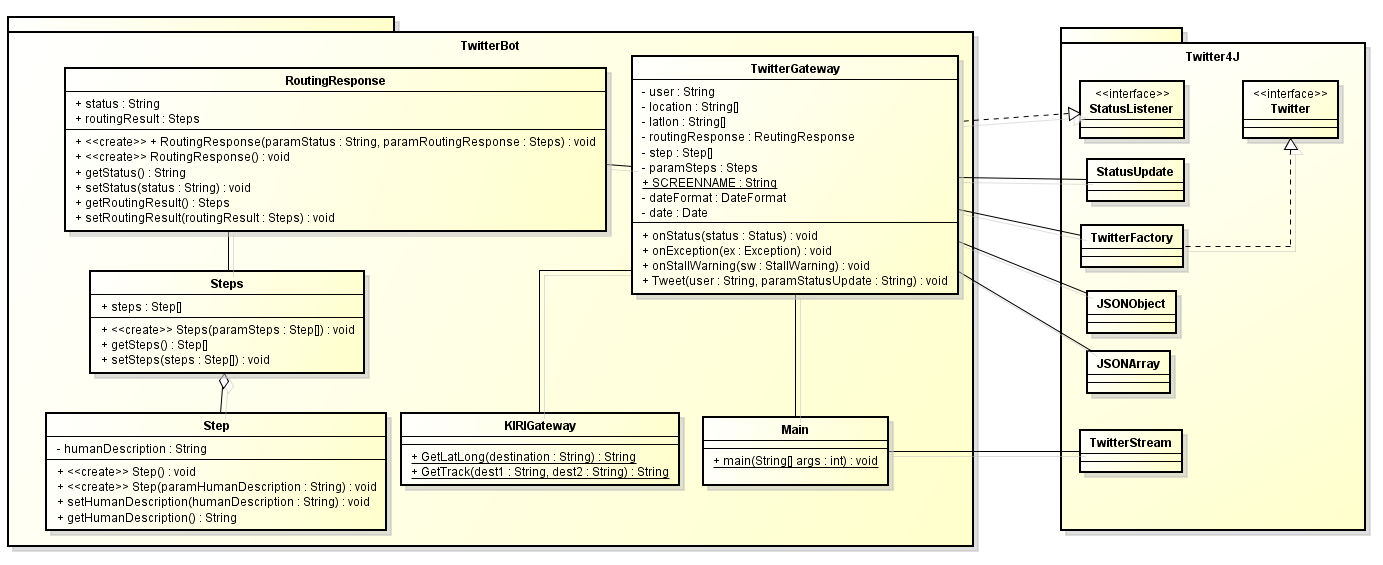
\includegraphics[width=1.00\textwidth]{C:/Skripsi/doc/DokumenSkripsi/Gambar/classDiagramSkripsi.PNG}
	\caption{Class Diagram Pembuatan Twitter Bot untuk Mencari Jalur Transportasi Publik}
	\label{fig:classDiagramSkripsi}
\end{figure}


\begin{itemize}
		\item Kelas Main, merupakan kelas yang berfungsi untuk membuat koneksi dengan Twitter ketika program dijalankan.
		
				\begin{itemize}
							\item Method
							
									\begin{itemize}
												\item public static void main(String[] args), merupakan method main untuk menjalankan program.
										
									\end{itemize}
				\end{itemize}
		
		\item Kelas Twitter Gateway, merupakan kelas untuk menangkap dan membalas Tweet. Kelas Twitter Gateway ini mengimplementasikan \textit{StatusListener}.
		
		
				\begin{itemize}
							\item Atribut
							
							
									\begin{itemize}
												\item String user, digunakan untuk menampung nama user.
												\item String location[], berupa \textit{array} yang digunakan untuk menampung lokasi awal dan lokasi tujuan.
												\item String latlon[], berupa \textit{array} yang digunakan untuk menampung koordinat lokasi awal dan koordinat lokasi tujuan.
												\item RoutingResponse routingResponse, merupakan atribut ??/ variabel?? yang digunakan untuk menampung hasil yang diberikan oleh KIRI API.
												\item Step[] step, berupa \textit{array} yang berguna untuk menampung langkah-langkah informasi perjalanan.
												\item Steps steps, merupakan atribut ??/ variabel?? yang berguna untuk menampung semua step.
									\end{itemize}
							
							\item Method
							
									\begin{itemize}
												\item public void onStatus(Status status), merupakan \textit{method} yang menangkap \textit{tweet} dan memproses \textit{tweet} tersebut. Ketika ada \textit{tweet} yang masuk, \textit{tweet} tersebut akan diolah isinya. Jika \textit{tweet} yang diterima merupakan \textit{tweet} untuk mencari jalur transportasi publik maka \textit{tweet} tersebut akan dimasukan ke atribut yang sudah disediakan yaitu \textit{user}, lokasi awal dan lokasi tujuan. Setelah mendapatkan lokasi awal dan lokasi tujuan barulah proses pencarian dimulai dengan menggunakan \textit{method GetLatLong} dan \textit{method GetTrack} yang terdapat di kelas KIRIGateway. Hasil pencarian akan dimasukan ke dalam atribut \textit{routingResponse}, \textit{step}, dan \textit{steps}. Setelah itu akan dilakukan pemanggilan \textit{method Tweet} untuk melakukan proses balasan.
												\item public void onDeletionNotice(StatusDeletionNotice statusDeletionNotice),
												\item public void onTrackLimitationNotice(int numberOfLimitedStatuses),
												\item public void onScrubGeo(long userId, long upToStatusId),
												\item public void onException(Exception ex), merupakan method yang berguna untuk menangkap \textit{exception}.
												\item public void onStallWarning(StallWarning sw),
												\item public void Tweet(String user, String paramStatusUpdate), merupakan method untuk melakukan \textit{tweet} balasan atau \textit{reply} yang ditujukan kepada \textit{user} tertentu. Twitter sendiri hanya dapat melakukan tweet dengan batas 140 karakter, oleh karena itu method ini akan mengatasi keterbatasan tweet tersebut dengan cara ??memecah-mecah?? tweet. Method ini juga akan memberi waktu yang sesuai dengan server di setiap akhir tweet, hal ini bertujuan untuk menghindari adanya duplikat tweet.
									\end{itemize}
				\end{itemize}
		
		\item Kelas KIRIGateway, merupakan kelas untuk memanggil KIRI API. Pemanggilan KIRI API ini digunakan untuk mendapatkan koordinat suatu lokasi dan mencari jalur transportasi publik.
		
		
				\begin{itemize}
							\item Method
							
							
									\begin{itemize}
												\item public static String GetLatLong(String destination), merupakan \textit{method} yang digunakan untuk mencari koordinat dari suatu lokasi. Hasil kembalian dari \textit{method} ini berupa \textit{latitude} and \textit{longitude} yang diberikan oleh KIRI API lalu diubah ke dalam bentuk \textit{String}.
												\item public static String GetTrack(String dest1, String dest2), merupakan \textit{method} yang digunakan untuk mencari jalur transportasi publik dari lokasi awal ke lokasi tujuan. Hasil kembalian dari method ini adalah langkah-langkah perjalanan dari lokasi awal ke lokasi tujuan dengan menggunakan transportasi publik.
									\end{itemize}
				\end{itemize}
		
		
		\item Kelas RoutingResult, merupakan kelas untuk menampung hasil kembalian dari KIRI API
		
		
				\begin{itemize}
							\item Atribut
					
					
									\begin{itemize}
												\item status, digunakan untuk menyimpan apakah status dari hasil pencarian.
												\item routingResult, digunakan untuk menyimpan langkah-langkah perjalanan.
									\end{itemize}
					
							\item Method
					
					
									\begin{itemize}
												\item public RoutingResponse(String paramStatus, Steps paramRoutingResult), merupakan \textit{constructor} dari kelas RoutingResult.
												\item public RoutingResponse(), merupakan \textit{constructor} dari kelas RoutingResult.
												\item public String getStatus(), merupakan \textit{getter} dari atribut status.
												\item public void setStatus(String status), merupakan \textit{setter} dari atribut status.
												\item public Steps getRoutingResult(), merupakan \textit{getter} dari atribut routingResult.
												\item public void setRoutingResult(Steps routingResult), merupakan \textit{setter} dari atribut routingResult.
									\end{itemize}
				\end{itemize}
		
		\item Kelas Step, merupakan kelas untuk menampung jalur perjalanan dari lokasi awal ke lokasi tujuan dengan menggunakan transportasi publik yang diberikan oleh KIRI API.
		
		
				\begin{itemize}
							\item Atribut
					
					
									\begin{itemize}
												\item String humanDescription, merupakan atribut untuk menjelaskan cara perjalanan yang bahasanya dimengerti oleh pengguna.
									\end{itemize}
					
							\item Method
					
					
									\begin{itemize}
												\item public Step(), merupakan \textit{constructor} dari kelas Step.
												\item public Step(String paramHumanDescription), merupakan \textit{constructor} dari kelas Step.
												\item public String getHumanDescription(), merupakan \textit{getter} dari atribut humanDescription.
												\item public void setHumanDescription(String humanDescription), merupakan \textit{setter} dari atribut humanDescription.
									\end{itemize}
				\end{itemize}
		
		\item Kelas Steps, merupakan kelas untuk menampung kumpulan step.
		
		
				\begin{itemize}
							\item Atribut
					
					
									\begin{itemize}
												\item Step[] steps, merupakan atribut yang berisi \textit{array} step
									\end{itemize}
					
							\item Method
					
					
									\begin{itemize}
												\item public Steps(Step[] paramSteps), merupakan konstruktor dari kelas Steps.
												\item public Step[] getSteps(), merupakan \textit{getter} dari atribut steps.
												\item public void setSteps(Step[] steps), merupakan \textit{setter} dari atribut steps.
									\end{itemize}
				\end{itemize}
\end{itemize}




\subsection{Sequence Diagram}

Pada sub bab ini, akan dijelaskan alur program dengan menggunakan \textit{sequence diagram} pada ~\ref{fig:diagramSequence2}

\begin{figure}[htbp]
	\centering
		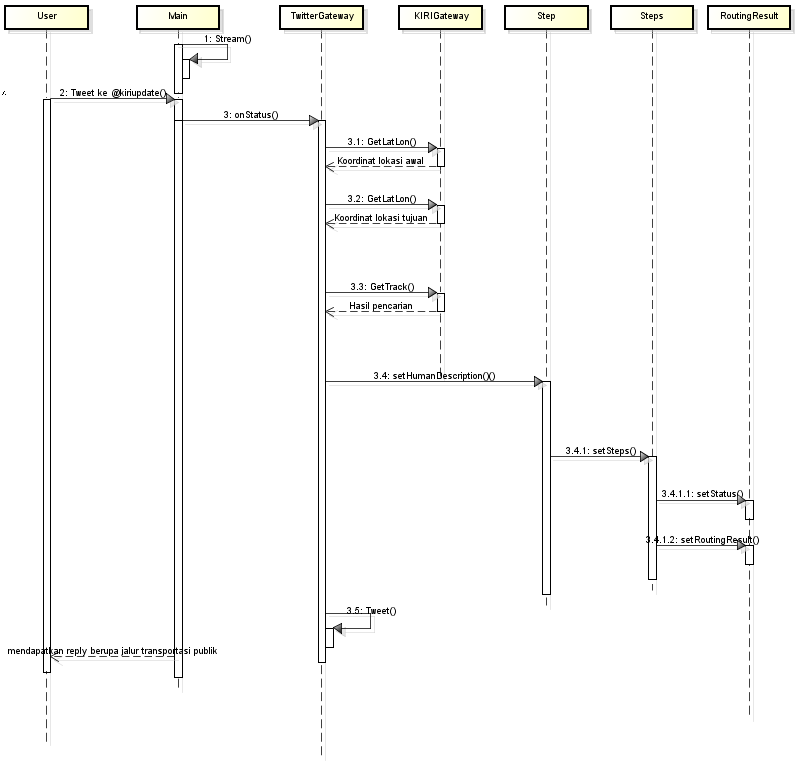
\includegraphics[width=1.00\textwidth]{C:/Skripsi/doc/DokumenSkripsi/Gambar/diagramSequence2.PNG}
	\caption{Sequence Diagram Pembuatan Twitter Bot untuk Mencari Jalur Transportasi Publik}
	\label{fig:diagramSequence2}
\end{figure}


Pertama, program akan melakukan \textit{streaming} pada saat kelas \textit{main} dijalankan. Kelas \textit{main} akan membuka gerbang untuk mengakses \textit{Twitter API}, dengan menggunakan \textit{Streaming} API aplikasi akan menangkap semua \textit{tweet} yang memiliki kata kunci @kviniink. Aplikasi akan terus melakukan \textit{streaming tweet} hingga aplikasi dinon-aktifkan.

Kelas TwitterGateway akan memproses \textit{tweet} ketika terdapat \textit{tweet} yang dirujuk (\textit{mention}) kepada @kviniink. \textit{Method onStatus} akan melakukan pengecekan apakah \textit{tweet} tersebut merupakan \textit{tweet} untuk mencari jalur transportasi publik atau bukan. Jika benar maka nama \textit{user} pengirim, alamat dari lokasi awal dan lokasi tujuan akan disimpan lalu akan dicari koordinat dari masing-masing lokasi menggunakan KIRI API. Proses mencari koordinat ini dilakukan oleh kelas KIRIGateway.

Kelas KIRIGateway akan memanggil \textit{method GetLatLon} untuk mencari koordinat suatu lokasi. Setelah didapatkan koordinat dari masing-masing lokasi maka kelas TwitterGateway akan mengolahnya terlebih dahulu dikarenakan hasil dari \textit{method GetLatLon} ini berupa JSON. Setelah itu maka hasilnya akan dikembalikan kepada kelas KIRIGateway untuk dicari jalur transportasi publik dari lokasi awal menuju lokasi tujuan menggunakan \textit{method GetTrack}. Hasil dari \textit{method GetTrack} akan disimpan pada atribut \textit{step, steps}, dan \textit{routingResult}.

Setelah selesai, langkah-langkah jalur transportasi publik siap di \textit{reply}. Proses \textit{reply} dilakukan oleh \textit{method tweet} yang terdapat pada kelas TwitterGateway. Tweet tersebut berisi tentang jalur transportasi publik dari lokasi awal menuju lokasi tujuan.\textit{Tweet} akan di-\textit{reply} satu per satu sesuai dengan banyaknya \textit{step} yang ada. Aplikasi akan terus melakukan proses tersebut hingga aplikasi dinon-aktifkan.

\subsection{Perancangan Antar Muka}
Aplikasi yang akan disusun ini memiliki antarmuka berbasis teks. Oleh karena itu, interaksi dengan pengguna dapat dilakukan melalui website atau aplikasi Twitter. Gambar ~\ref{fig:Homepage Mobile Twitter} adalah tampilan antar muka dari Twitter yang diakses melalui mobile. Dari situlah, pengguna dapat melakukan tweet untuk mencari jalur transportasi publik. Tweet dilakukan dengan cara menuliskan tweet kepada user @kviniink.

\begin{figure}[htbp]
	\centering
		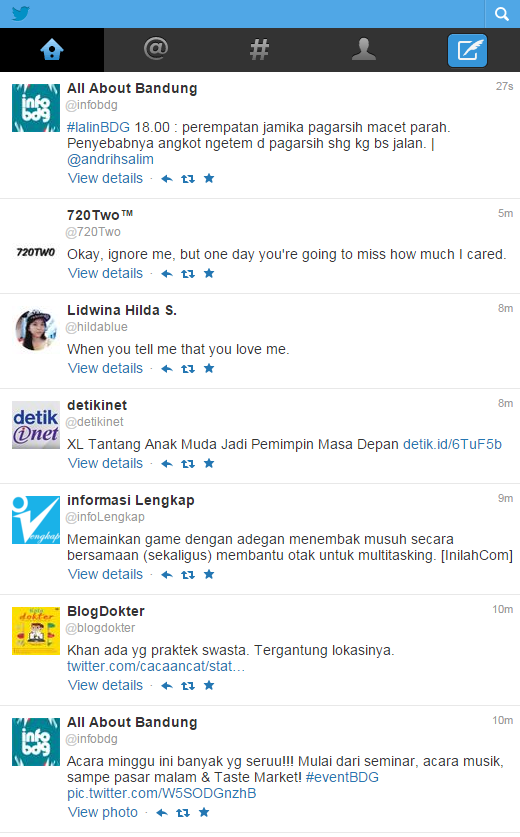
\includegraphics[width=1.00\textwidth]{C:/Skripsi/doc/DokumenSkripsi/Gambar/Homepage Mobile Twitter.PNG}
	\caption{Homepage Twitter versi mobile}
	\label{fig:Homepage Mobile Twitter}
\end{figure}

Gambar ~\ref{fig:Textbox Mobile Tweet} menunjukan menu untuk melakukan tweet. Pertama, format yang dimasukan harus benar. Format dari penulisan tweet adalah "`lokasi awal"' to "`lokasi tujuan"'. Ketika user melakukan tweet maka Twitter Bot untuk mencari jalur transportasi publik akan menangkap tweet tersebut dan akan memproses tweet tersebut, rancangan dari hasil tangkapan tweet dapat dilihat pada gambar ??. Sedangkan rancangan dari hasil pencarian dapat dilihat pada gambar ??.

\begin{figure}[hp]
	\centering
		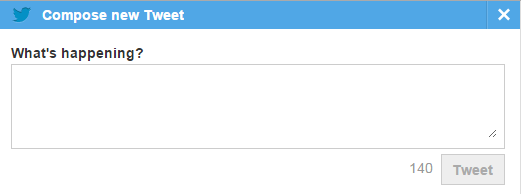
\includegraphics[width=1.00\textwidth]{C:/Skripsi/doc/DokumenSkripsi/Gambar/Textbox Mobile Tweet.PNG}
	\caption{Tampilan untuk melakukan tweet}
	\label{fig:Textbox Mobile Tweet}
\end{figure}




